\documentclass{article}
\usepackage[utf8]{inputenc}
\usepackage{graphicx}
\usepackage{subcaption}
\usepackage{amsmath} % For matricies 
\usepackage[export]{adjustbox}
\usepackage[hidelinks]{hyperref}
\usepackage{setspace}
\usepackage{pdfpages}   % To add record of supervision as pdf

% change reference style to [1], remove stupid sorting, language changed so date in ddmmyyyy
\usepackage[backend=biber, style=numeric, sorting=none, language=australian]{biblatex}
\addbibresource{References.bib}


%----------------------------------------------------------------------------------------
%	TITLE SECTION
%----------------------------------------------------------------------------------------

% 10.1.1 Title Page (Compulsory)
% A title page shall be provided for each binding volume of the dissertation, and shall give the following information:
% (a)	the full title of the dissertation and the subtitle if any;
% (b)	the full name of the author (and student number);
% (c)	the month and year of submission (e.g. “September 2020”);
% (d)	“Project Dissertation submitted to Swansea University in Partial Fulfilment for the Degree of Master of Science”;
% (e)	the department and the university where the project was conducted
% 	(i.e. Department of Computer Science, Swansea University).


\newcommand{\horrule}[1]{\rule{\linewidth}{#1}} % Create horizontal rule command with 1 argument of height
\title{
\begin{Huge}\textbf{Detecting User Engagement Using Mouse Tracking Data} \end{Huge} \\% The assignment title
\vspace{70px}

\includegraphics[width = 65mm]{Images/SwanseaUniversity}\\[8ex]
%\begin{large} \textsc{\textbf{MoHo. Khaleqi}} \end{large} \\ % Your university, school and/or department name(s)
\vspace{10px}
\normalfont \normalsize 
\begin{normalsize}Department of Computer Science \end{normalsize}\\  % Your university, school and/or department name(s)
\begin{normalsize} Swansea University \end{normalsize} \\ % Your university, school and/or department name(s)
\vspace{60px}
This dissertation is submitted for the degree of\\
\textit{Master of Science}
\vspace{20px}
}
\author{David Saunders (910995)} % Your name
\date{September 2020} % Today's date or a custom date
\newpage

% \title{Detecting User Engagement Using Mouse Tracking Data}
% \author{David Saunders (910995)}
% \date{September 2020}

\begin{document}
\pagenumbering{gobble}  % Turn off page numbering
\maketitle
\pagebreak

% ******************************* Thesis Declaration ***************************
\null\vspace{\fill}
\vspace{2cm}

\begin{center}
    \textbf{Declaration}
  \end{center}


This work has not previously been accepted in substance for any degree and is not being concurrently submitted in candidature for any degree.

\vspace{1cm}
\begin{flushright}
 David Saunders\\
 September 2020
\end{flushright}

\begin{center}
    \textbf{Statement 1}
  \end{center}

This dissertation is the result of my own independent work/investigation, except where otherwise stated. 
Other sources are acknowledged by giving explicit references. 
A bibliography is appended.

\vspace{1cm}
\begin{flushright}
 David Saunders\\
 September 2020
\end{flushright}

\begin{center}
    \textbf{Statement 2}
  \end{center}

I hereby give consent for my dissertation, if accepted, to be available for photocopying and for inter-library loan, and for the title and summary to be made available to outside organisations.

\vspace{1cm}
\begin{flushright}
 David Saunders\\
 September 2020
\end{flushright}


\vspace{\fill}
\pagebreak

% The abstract is a good start. It's better to be more specific about
% what your thesis is about. So, the first sentence should be something
% like "this project explores the use of HMMs to determine if users are
% paying attention during a crowdsourced study." I would also remove the
% last sentence. That's more of a future work idea.

% Basically they want an abstract, renamed as a summary.
% 10.1.2 Summary (Compulsory)
% There shall be a summary of the dissertation not exceeding 300 words. 
% The summary shall provide a synopsis of the dissertation and shall state clearly the 
% nature and scope of the work undertaken and of the contribution (if any) made to the
% knowledge of the subject treated.

%\renewcommand{\abstractname}{Summary}

\begin{abstract} 
    %TODO: Update with results from secondary model and say how you doubt it.
    %Potential abstract.
    %This project explores the use of Hidden Markov Models to explore users mouse cursor data while performing a task.
    This project explores the use of Hidden Markov Models to determine if users are paying attention during a crowdsourced study.
    The users are split into two distinct groups, online crowdsourced users, and lab study users.
    It is proposed that the lab study users were paying attention, and the crowdsourced users may or may not be paying attention.
    By using observed data recorded from user's mouse cursor it is possible to model both groups interaction with the system with separate Hidden Markov Models.
    Some user's interactions seem misplaced compared to their groups.
    These are reclassified with the aim of changing the groups of users from lab study or crowdsourced, to users paying attention and not paying attention.
    It was found that potentially between 4.4\% and 50.9\% of the crowdsourced users were paying attention, which reflect the known inaccuracies of crowdsourcing data.

    % These results require further research with a properly labelled dataset to confirm any findings.
    % I would also remove the last sentence. That's more of a future work idea.
\end{abstract}
\pagebreak

\tableofcontents
\pagebreak

% From the official swansea uni template.
%\input{list_of_tables_and_figures} 

\listoffigures
\listoftables
\pagebreak

% Toms layout
% Motivation
% Related Work
% Implementation
% Results
% Conclusion

\onehalfspacing

% motivation: mention why paying attention is important
\section{Motivation}
\pagenumbering{arabic}

% Why is it important
% Why is it a hard problem/problems
% Why other authors have failed
% My contributions are - bullet list
% My idea to fix it

% Original before copying from project specification

% Detecting use engagement is an important science across multiple disciplines.

% Find a study that says during any task / any crowdsourced task X\% of people are not paying attention.
% This could jeopardise the results from any online if we cannot be sure users are actually paying attention to the task they are being paid to complete. 

% It is a hard problem because, among other things I will touch on, it is hard to quantify exactly what user engagement is exactly.
% One author defined it as 'XYZ' [look at my previous work for references].

% However the previous authors have failed to detect and measure user engagement as X,Y,Z.


% TODO talk about some of the papers Tom links in his paper, such as  
% Finding Waldo: Learning about users from their interactions
% His paper literally outlines my project so defo worth exploring what he says.

% COPIED DIRECTLY FROM PROJECT SPECIFICATION

%https://academia.stackexchange.com/questions/44784/how-to-explain-things-in-the-motivation-section-of-a-mathematical-paper-without
% People have wondered about how to better understand frobs ever 
% since Richard Feynman first used them to pick the locks in Los Alamos. 
% Although X, Y, and Z attempts have been made, none of them got very far
%  because they were all green-colored. 
%  In this dissertation, I examine an alternate path, reducing the problem
%   of frobs to the simpler system of greebit-space by means of an 
%   innovative application of wibbling. 
%   These results bring us one step closer to solving the problem of frobs, 
%   and how they can be better used to quickly and cheaply pick locks.

% Paragraph 1 - Initial motovation
Crowdsourcing is a method of collecting responses from tasks that require human intelligence to complete. 
One such example of a crowdsourcing service is Amazon's Mechanical Turk \cite{AmazonTurk}.
Here users known as ``Turkers'' complete tasks in exchange for a small financial incentive. 
%Crowd-sourcing marketplaces like Amazon's Mechanical Turk are popular services that provide a method for researchers to get participants to complete human intelligence tasks \cite{paolacci2010running}. 
A common use for this technology is to label data for use in training for machine learning algorithms \cite{chang2017revolt}.
They can also provide a cheap, scalable method for scientists to gather responses in research \cite{paolacci2010running}.

% Paragraph 2 - Inter disciplinary
The use of gathering responses using Amazon's Mechanical Turk and other crowdsourcing alternatives are becoming prevalent across disciplines.
It is commonly used in conducting clinical research \cite{chandler2016conducting} and it is estimated that almost half of all cognitive science research involves the use of crowdsourcing services to collect data samples \cite{stewart2017crowdsourcing}.
The creation of an easy to implement method to measure user engagement would massively help researchers to increase reliability of their research.

The level of user engagement, attention, and low-quality responses can all be issues when gathering data from participants with distributed approaches \cite{ipeirotis2010quality}.
The primary motivation of this project is to develop a system of potentially identifying if a crowdsourced user is paying attention during a task.


% Paragraph 3 - Motivation
Research has been conducted on how the accuracy and attention of crowdsourced tasks can be increased.
% Look at these papers to see how they classified attentions.
Methods such as offering financial incentives \cite{ho2015incentivizing} and engaging a user's curiosity \cite{law2016curiosity} have been found to motivate workers into performing better at crowdsourced tasks.
Despite the research there is still debate as to which method is superior.
If user engagement can be effectively identified, then the best method of ensuring user engagement could be found using this method.

% Paragraph 4 - Why measuring attention is hard and why obvious solutions wont work. 
% It's worth spending some space on why this problem is hard and why any obvious solutions won't work

%Maybe it is hard to quantify attention as it is hard to do so.
%Measuring attention is hard and obvious solutions wont work.
Measuring user engagement is well studied in the field of web analytics \cite{peterson2008measuring}.
However, the existing methods of reporting and analysing website data cannot be easily applied to crowdsourced tasks.    
Characteristics such as session duration and customer satisfaction are used as proxies for engagement.
However, a longer session doesn't necessarily mean a more engaged user and customer satisfaction is not applicable for crowdsourced tasks.
Therefore, existing solutions will not work and now methods must be evolved.

% TODO: Talk about the past of crowdsourcing and give more details about it
% Give users who know nothing about the topic guidance on what everything even is.

\subsection{Background}
% TODO: Maybe link to Toms paper too

% TODO Have this section finished soon and have Meg look over it: 04/09/20

The work in this project is built on data gathered from a previous study;
\textit{``A comparison of user interactions in lab and crowdsourced
studies''} \cite{gruber2017thesis}.

%TODO: Was it a data vis paper?
The study was centred in the field of data visualisation.
The paper explored whether an alternative more detailed interface could be used help improve a user's effectiveness at completing a task.
The task simulated an investment scenario, the aim was to maximise the return of a collection of stocks over several iterations. 

\begin{figure}[ht]
    \centering
    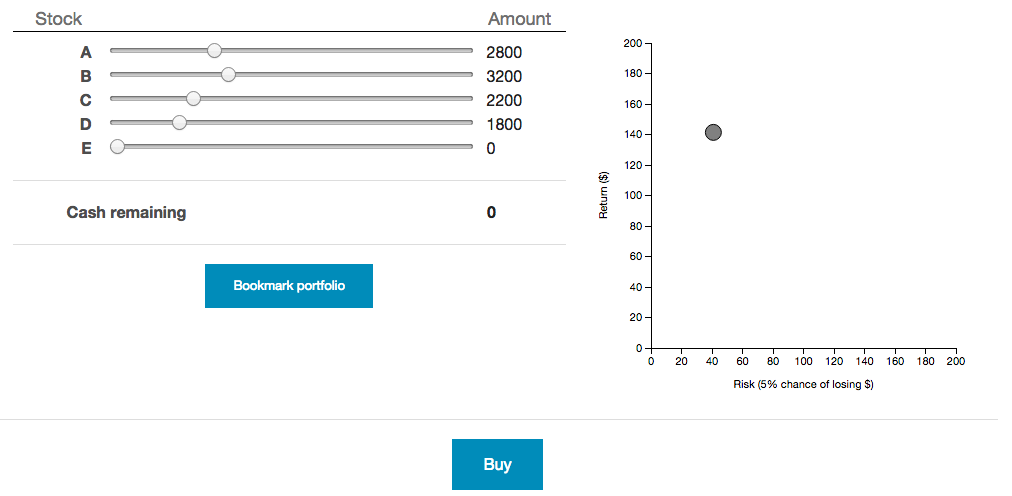
\includegraphics[scale=0.35, frame]{Images/interface.png}
    % TODO: Find the right interface, current interface doesn't match whats in his paper.
    \caption{The main interface of the lab study, with the risk and return of stocks to the right and allocation sliders to the left.}
    \label{fig:interface}
\end{figure}

%The experiment identified two users groups, risk fixers and sweet spotters, based on their response in a questionnaire.
Figure \ref{fig:interface} shows the main interface of the lab study, with the risk and return of stocks to the right and allocation sliders to the left.
Users were asked to invest their money by putting it into varying amounts of stocks.
The 5 stocks were labelled from A to E.
Depending on the makeup of the user's stock portfolio, the plot would update showing the return and risk of their portfolio.
They were then asked to confirm their choice by buying these stocks.
This process was repeated for 5 steps, where after each step the user's portfolio value with increase based on their previous investment decisions. 

% TODO get picture of global sa sl both
\begin{figure}[ht]
    \centering
    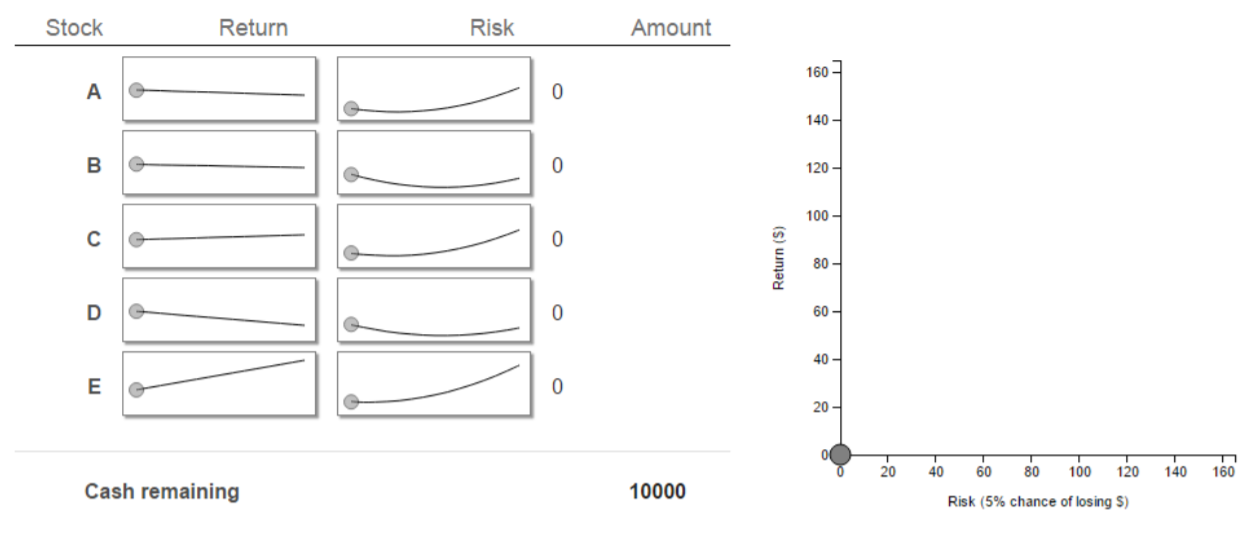
\includegraphics[scale=0.45, frame]{Images/interfaceSA.png}
    % TODO: Find the right interface, current interface doesn't match whats in his paper.
    \caption{The alternative user interface of the lab study.}
    \label{fig:interfaceSA}
\end{figure}

Figure \ref{fig:interfaceSA} shows that the sliders representing each stock are split into two separate sliders, showing the return and the risk of the stock.
Additionally, the sliders are no longer one dimensional, both sliders are two dimensional line charts.
The assumption of the study was that these extra visualisations would help users to maximise the value of their portfolio.

\begin{table}[ht]
    \caption{\label{table:studies} Data collection methods used in the study \cite{gruber2017thesis}.}
    \small
    \begin{tabular}{lll}
        \hline
        Data collection method & Number of participants & Were participants paying attention? \\    \hline
        Lab study              & 18                     & Yes                                 \\
        Crowdsourced task      & 370                    & Unknown                             \\    \hline
    \end{tabular}
\end{table}

Table \ref{table:studies} shows the two different ways in which data was collected.
Only 4.6\% of the data was gathered in person, with the most of responses being crowdsourced using Amazon's Mechanical Turk.
The difference in number of participants shows one of the reasons crowdsourcing is popular. 
It is much easier to crowdsource responses than it is to organise an in-person lab study.
Participants from the lab study were heavily monitored to ensure they were engaged, focusing on the task.
The crowdsourced participants were not monitored so it is unknown if they were engaged with the task, without further analysis.

The study was inconclusive in proving that the alternative interface design had a meaningful effect on the success of a user's portfolio.
Therefore, for the purpose of this project the distinction of which interface a participant was using is ignored.
Additionally the rationale is that regardless of which variant of the interface was being used the participant would be paying attention.
There is likely to have crowdsourced users who are engaged and some that are not engaged regardless of which interface is used.
While there will be differences in users mouse data depending on the interface, I hypothesise that the difference will not be as large as the difference between users that are engaged or not engaged. 

\subsection{Initial attempt}

One naive assumption might be that a users attention level might be inferred from the time taken to complete the tasks.
Exploration of the data showed that the division of users may not be so straightforward, shown in Figure \ref{fig:scatterplot}.
% TODO add plot of lengths vs time for different groups.

\begin{figure}[!h]
    \centering
    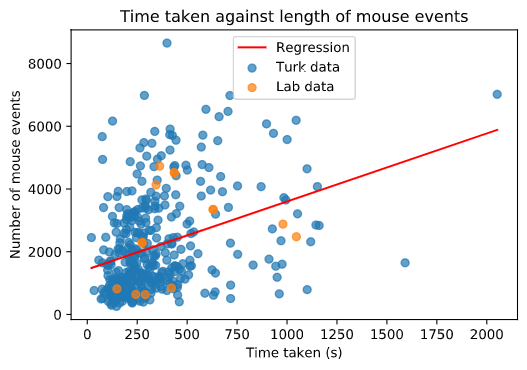
\includegraphics[scale=0.55]{Images/TimeTaken-Mouse-Events.png}
    % TODO: Find the right interface, current interface doesn't match whats in his paper.
    \caption{Scatterplot of users.}
    \label{fig:scatterplot}
\end{figure}

The lab and turk user classes cannot be separated by a simple metric of their data, such as length of events sequence and time to complete task.
This eliminates the option of using distance based machine learning approaches such as K Nearest Neighbours or a Support Vector Machine as there is no relationship between such simple features.
It should be noted that length of events sequence and time are correlated with a Pearson's correlation of $0.344$.

% Meg Removed
% As a rule of thumb, we can say that correlations below 0.3 have no relationship, and values between 0.3 and 0.5 have a weak relationship \cite{mindrila2017scatterplots}.
% This means the two features are weakly correlated, but correlated nonetheless.
% This means that one of these features may be a good substitute for the other and that having both may be redundant.

\subsection{Contributions}
% The contributions are 1,2,3 (everyone likes 3s)
% Take aways of how it will help them.

% INITIAL CONTRIBUTIONS     - Removed as they dont match the actual contributions of the diss
% In this project my contributions to fix it are, 
% -a system to classify users, 
% a way of visualising their mouse paths, 
% ways to directly and quantitatively compare different users, 
% and a multistage semi-supervised based binary classification output to answer the question of 'are users engaged'.

% TODO: Maybe an initial introduction before the contributions start.

The contributions of this paper can be summarised as follows:

\begin{enumerate}
    \item The development of a system to model a study participants mouse data, and to detect outliers from groups of users.
    \item The creation of visualisations to explore participants mouse data.
    \item The creation of methods of generating new data given small amounts of existing data.
  \end{enumerate}

\subsection{Hypothesis}

The main hypothesis of this project is that the lab study participants were paying attention and at least some of the crowdsourced participants were.
Additionally I hypothesis that whether a user is engaged in the task and paying attention can be inferred from their mouse data.
Any outliers from the crowdsourced data that appear to be more similar to the lab data will be examined.
The outliers can then be reclassified as potentially paying more attention than there peers.

There is the question of are the differences in data from the two groups caused by their engagement, or is it due to other factors.
The main difference between a crowdsourced user and a lab study is their location completing the study.
This relates directly to their engagement as we know the lab study participants were always engaged since they were monitored.
Therefore, I think it is reasonable to assume that it is plausible that any differences in data are due to a participants engagement.

\section{Related Work}

% Convince the reader you've done enough work and research in the area.
% Convince them it was hard and the topic is hard so you need to help.
% You've tried other peoples techniques.

% From MEG:
% In this section I will discuss XYZ and how it related to my project at whole.
% I cover the topics of eye tracking, cursor tracking, and ...
% Other topics that could have been included but weren't are ...

In this section I will discuss the related work to my project.
This will include more general research in the fields of tracking user's mouse data and detecting a user's engagement.
Works about crowdsourcing data are found which are key in understanding the background of this project.
Machine learning techniques, and previous projects that have the possibility of being used in this context are also researched.

%   rel work: often I have an intro paragraph about how this work spans
%   categories a, b, and c (and briefly why) and then I have subsections
%   like you do for each category

% Taken from project specification

% Dont really link to engagement 
\subsection{Eye tracking}

Non-verbal information such as eye tracking may be used to detect user's level of engagement \cite{lala2017detection}.
Vision is one of the most powerful human senses, so it has the potential to give a good measure of user engagement. 
The methodology of eye tracking is that we move our eyes to focus on particular areas that we want to see in more detail and divert our attention to that area \cite{duchowski2007eye}. 
% duchowski2007eye is a VERY important piece of literature for the field, over 4000 citations
Thus, tracking a user's gaze can provide insight into which part of a system they're engaged with, and how much so.

\begin{figure}[ht!]
    \centering
    \centerline{
        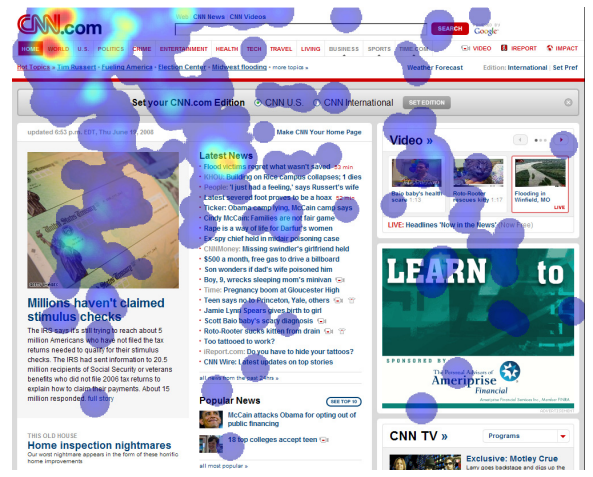
\includegraphics[scale=0.6]{Images/EyeHeatmap.PNG}
    }
    \caption{Eye tracking visualisation showing popular locations of users eyes on a webpage. Red areas are more frequently looked at than blue areas \cite{buscher2009you}.}
    \label{fig:eyetrack}
\end{figure}

Eye tracking data can be used to show interface elements that users focus their attention on, shown in Figure \ref{fig:eyetrack}. 
From this data researchers were able to predict the amount of attention elements of the page would receive.
By observing what parts of an interface users are interacting with we can determine what a user is engaging with \cite{buscher2009you}.

Eye-tracking has been used, and found success in novel applications such as recording the engagement of users when playing a game. 
Tracking users eye movements helped game designers understand how users can recognise interactable game objects and could be used to investigate problematic game design issues \cite{renshaw2009towards}.

%TODO: I mention researchers names here, but nowhere else?
% Make consistant
Researchers are able to extract features from a users eye tracking data to determine their cognitive state in a problem solving exercise \cite{eivazi2011predicting}.
Features such as ``mean fixation duration'' and ``total path distances'' were engineered, and users were split into classes based on their performance. 
Given a user feature set and their performance class it was able to classify their cognitive state during the task with a 87.5\% accuracy with a Support Vector Machine.

There are a plethora of verbal and non-verbal behavioural cues used by teachers in educational settings to detect engagement, with gaze being identified as one of them \cite{szafir2012pay}.
The behavioural cues could not be recorded directly by a computer, instead EEG signals measured from a headset were used to measure engagement.

Eye tracking is not however a perfect solution and its limitations have been well documented. 
Tracking subjects eyes with a good degree of accuracy requires the use of expensive, intrusive equipment that frequently needed recalibrating \cite{richardson2004eye}. 
Therefore, these limitations rule out eye tracking to explore user engagement in my research.

\subsection{Mouse cursor tracking}
% Copied straight from CSCM10 Initial Report
% Mouse cursor tracking

There is a direct correlation between a user’s gaze and their cursor position. 
The position can be considered a ``poor man’s eye tracker'' as it has been found that eye gaze match mouse position 69\% of the time \cite{cooke2006mouse}. 
Mouse movement data can be collected without the drawbacks of eye tracking and with more automatic methods, meaning more data can be collected, and on a larger scale \cite{demvsar2017quantifying}.
Therefore, it can be said that mouse data can be used as a good alternative to eye tracking data.

%Mouse activity can be used as input to a neural network and output a quantifiable level of activity for a webpage. 
By using mouse data, it is possible to unobtrusively record a user’s normal use of a web browser without disturbing their experience \cite{goecks2000learning}.
% Above paper touches on one of the big advantages of measuring user engagement from mouse data, it is unobtrusive! We can monitior them in the background 
It has also been found that users tend to follow the text they are reading with the mouse cursor \cite{liu2007detecting}. 
It can be determined what paragraph of a page was being read with an accuracy of 79\% by using mouse cursor data \cite{hauger2011using}. 

Other methodologies explored ways of classifying user engagement from eye and cursor data, however it is also possible to predict user's attention and user frustration in complex webpages \cite{navalpakkam2012mouse}.
Not all studies agree that mouse cursor is always a good approximation for eye data. 
Some have found that distinct cursor behaviour exists depending on the task a user is completing.
This means that the relationship between eye gaze and mouse position is more nuanced than measuring only mouse data \cite{huang2012user}.

The benefits of tracking users mouse cursors, lead me to believe it will be a suitable attribute to measure from users for this project. 

% \subsection{Machine learning techniques}
% I've given a high level overview of the existing literature, here I will be more in depth as to the algorithms and techniques relevant to this project.

\subsection{Crowdsourcing Cheating}
% TODO: find a ML project on detecting low quality responses from surveys.

% https://www.researchgate.net/publication/228440813_Increasing_cheat_robustness_of_crowdsourcing_tasks


The inaccuracies of responses when crowdsourcing results is a well-established issue.
Users are paid per job complete, giving them incentives to complete tasks as fast as possible to maximise their income.
Workers speed up task by submitting incorrect results, or by failing to perform the task correctly \cite{hirth2013analyzing}.
These workers can be labelled as cheaters, as their contributions are unusable.
% This is a really good paper, should defo talk more about it.


% Expand on this greatly.
The crowdsourcing platform Crowdflower created an integrated method of detecting cheating to address this issue.
This method was used effectively when using human workers to help label datasets \cite{quinn2010crowdflow}.
Tasks for which the answer is known are periodicity asked to the user, and the accuracy is measured.
Once a user has completed a number of tasks over a threshold value then their accuracy on the known tasks is assessed.
Of this accuracy is deemed to be unacceptable then the results from that user are ignored, and they are prohibited from contributing any more.
This system has the drawback of taking more time and being more expensive than with no cheat detection method.
Out of the 15 unique users that completed some of the tasks 9 of them where labelled as cheaters, presumably using scripts to randomly select answers.
This allowed them to create a much larger volume of responses than any legitimate users, with 91\% of the results coming from cheaters.

Crowdsourced tasks can be classified as Closed Class tasks and Open Class tasks, with each having unique cheating approaches \cite{eickhoff2013increasing}.
Closed class questions are more common, requiring workers to choose an answer from a predefined list.
This includes check boxes, buttons, multiple choice questions, and importantly to this project, sliders.

Randomly picking answers is the most common cheating attempt, this can be detected by comparing a suspected users responses with a user known to not be cheating or comparing with all other workers answers.
% Can add other cheating attempt if we want to.
Open class questions are much easier to cheat, these involve giving a user much more freedom to complete a task.
Typically, workers may be given blank text fields to fill in, or blank canvas' to draw on.
Standard cheating approaches involve leaving the fields empty, or repeatedly entering the same text.
These approaches can be easily detected.
More advanced attacks copy domain specific text copied from the internet, which is difficult to detect. 

\subsection{Spam detection}
% TODO: add section on SPAM detection, they're similar in a way?

Spam detection can be thought of as a binary classification problem.
Given a document such as an email, review, or tweets can the non-spam be separated from the spam.
Spam documents can be though of as unwanted nuisance such as an advertisement, scam, and hoaxes \cite{sasaki2005spam}.
 
This shares similarities with crowdsourcing cheating, both involve trying to identify genuine wanted data from other unwanted data.

The detection of spam email is a classic machine learning problem.
Unsolicited spam emails are sent out in such large quantities, in part due to how cheap they are to send.
Bayesian classifiers such as Naive Bayes obtain good results and are being used by multiple spam detecting softwares.
Other successful techniques include Support Vector Machines and test clustering methods such as measuring the cosine similarity of new mails and classify them using k-means \cite{sasaki2005spam}.

Spam reviews are becoming a big issue for E-commerce websites such as Amazon.
There are obvious financial incentives to spam reviews.
A product with many positive reviews is more likely to be purchased than a similar product with many negative reviews.
Therefore spam reviews can directly lead to increased profit.
Many spam reviews are duplicates, different uses posting the same positive review or a product, or multiple products.
Using features from user and review data it was possible to use logistic regression to achieve an average AUC value of 78\% \cite{jindal2007review}.

The social media platform twitter has been experiencing issues due to large amounts of spam data.
Using twitters API can give information regarding the friend and follower status between tweeters.
This can be used to detect cases of unknown spam accounts contacting genuine users.
Again a Bayesian classifier was found to have the best overall performance \cite{wang2010don}.   



% these subsections below are old
% probably pointless as they're just some ML techniques and not backgroud

\subsection{Semi Supervised Learning}
This will be a key aspect of the project as we only have definitive labels for part of our data.
This reflects the challenges of real-world data, where the quantity of unlabelled data is much greater than labelled data.
% Find reference that says X amount of data is labelled.

% https://sci-hub.tw/10.2200/s00196ed1v01y200906aim006 'Introduction to Semi-Supervised Learning' good paper that ive referenced below.
Semi-supervised learning is the study of combining both labelled and unlabelled data to improve machine learning techniques \cite{zhu2009introduction}.
One of the most popular semi-supervised learning techniques are Semi-Supervised Support Vector Machines (S3VMs).

%Mention abbreviation semi supervised learning (SSL)

%TODO: Add back in at somepoint
%Reference \cite{zhu2005semi} as it looks to be massively influential with 4,000 google scholar citations.


All of the data used in this dissertation is labelled.
The data belongs to two classes, a crowdsourced turk user class, or a lab study user class.
However, on the other hand the data is not labelled for the task I would like to explore.
The goal of this project is to identity which users were paying attention.
We have assumed that we can infer that lab study users will be paying attention, so we can say that those samples are labelled.
However, the rest of the samples we have which are all of the online data are unlabelled.
Therefore, this is a kind of semi supervised learning problem where we only have a small percentage of our samples labelled, and only confident labels for one class.
% TODO: (See if a paper on this exists, semi supervised binary classification with only labels for one class.)
% Do a literature review type of thing where I review semi supervised learning, talk about methods and how they can be applied to what I'm trying to do.

Semi supervised learning has already been applied successfully to the field of user engagement.
During a 2017 study video data of secondary school children was recorded during a set of tasks, with the aim of classifying pupils between the states of `Engaged' and `Disengaged' \cite{nezami2017semi}.
Rather than annotate all data by hand which would be very time intensive, 1000 frames of video were selected at random and hand labelled.
This led to a split of data labelled 563 engaged and 437 disengaged.
AU facial recognition features were extracted from the pupils faces in the video frames, and important features decided with a Principal Component Analysis method to keep features totalling 95\% of the variance.

Their chosen method of semi supervised learning is a Safe Semi-Supervised Support Vector Machine.
This variant of a Semi Supervised Support Vector Machine finds a better separator when there is a small volume of labelled data, but a large volume of unlabelled data.
The SSL model was trained with numbers of labelled data from 50 to 500, and an equal number of samples from both classes.
The AUC metric ranged from 0.65 to 0.733 depending on the quantity of labelled data used, outperforming a traditional SVM.

Unfortunately, as shown in figure \ref{fig:scatterplot} the data here cannot be spatially separated and therefore any SVM would not be successful on the data.
This is because Support Vector Machines are large margin classifiers, they work by finding a hyperplane that maximises distance from datapoints of different classes \cite{campbell2000query}. 
It is still useful however to see how semi-supervised learning has been applied to the field of detecting user engagement and how it has been successful.

% Removed N-Grams section as wasn't used in the final product. 
%\subsection{N-Grams}
%This paper has a nice scientific explanation of n-grams \cite{tomovic2006n}.
%Either cite this paper or more likely look at their reference for n-grams and cite that.
%   

\subsection{Hidden Markov Models}
% Does this belong in the related works section? seems more like implementation section.

% explanation from scratch: https://towardsdatascience.com/hidden-markov-model-implemented-from-scratch-72865bda430e



% Wikipedia definition:
% "Hidden Markov Model (HMM) is a statistical Markov model in which the system being modeled is assumed to be a Markov process – call it X – with unobservable ("hidden") states. 
% HMM assumes that there is another process Y whose behaviour "depends" on X.
% The goal is to learn about X by observing Y." Wikipedia

% file:///C:/Users/DJSau/Downloads/588dfc2633c3cd86ab3faba2a44a8e4ceb63.pdf
% AN INTRODUCTION TO TEXT MINING
% 2.2.1 Hidden Markov Models has a nice concise description.

A Hidden Markov Model will be the main statistical modelling technique used in this dissertation.
In this section I will give an overview of what they are, and how they have been used in related projects.
A Hidden Markov Model (HMM) is a statistical modelling technique based on the Markovian process. %Reference?
That is the states of the system follow the rules for a Markov process, meaning every state depends only on the previous state of the system.
It assumes that we cannot observe a system directly, but only see observations from it.

%Cite diagram from here https://www.researchgate.net/publication/245563174_State_Dependence_in_Lane-Changing_Models/figures?lo=1
\begin{figure}[ht!]
    \centering
    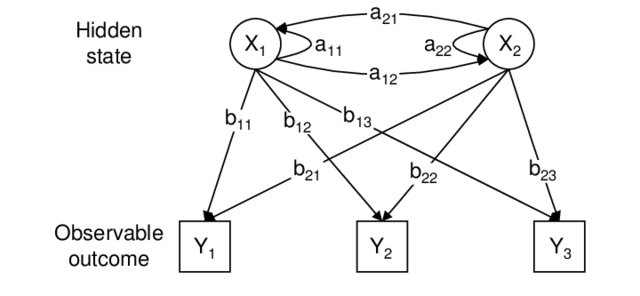
\includegraphics[scale=1.5]{Images/HMM-Paper-Diagram.png}
    \caption{Diagram of an example Markov Chain model \cite{choudhury2007state}.}
    \label{fig:Markov}
\end{figure}
% Alternatively make a similar looking diagram from scratch in Google drawings.

HMMs can be defined with the parameters $(Q,A,O,B,\pi)$ \cite{jurafsky2018speech}.
$Q$ is the set of hidden states of the system, the cardinality of which is normally selected empirically \cite{ibe2013markov}.
$A$ is a transition probability matrix, a square matrix of shape $|Q|\times|Q|$.
This matrix consists of the probabilities of transitioning from one state to another with each row and column representing a state in $Q$
, and the main diagonal of the matrix representing a self-transition.
$O$ is the sequence of observations from the system.
$B$ is the emission probabilities of the model, these give the probabilities of each observation coming from each state.
$\pi$ gives the initial probability distributions of the system.
It is a set with the same cardinality as $Q$, where each item in $\pi$ relates to the probability of the model starting in a specific state.

% Explain this better, but im not really sure myself
% Had a cursor interface similar to this, but not sure what they did lol.
%HMMs have had success in modelling user behaviour when completing a simple task \cite{ibe2013markov}.

%TODO: PUT THESE BACK IN AND EXPAND ON THEM!!!
%Paper Tom send me about HMM for text classification that I might be able to use \cite{collins2016tagging}.

%Paper claims to use HMM for spam detection, I think they actually just use it to detect misspellings of words or something which is used by spam to hide from filters \cite{gordillo2007hmm}.
%Probably could find a better spam detecting HMM, I just like how this almost does something different from the title, which my diss will end up doing.

%This paper was recommended by someone on stack overflow as an old influential paper in the field with tens of thousands of references \cite{rabiner1989tutorial}.
%Called a tutorial on HMM and it's so old so original source. 
%Would definitely be good to reference if I include any of the mathematics behind HMMs. 

% Have figure caption like this, looks professional and really good.
% https://miro.medium.com/max/556/0*s4wQ8nTIb2122-9s.png


Figure \ref{fig:Markov} shows the components of a Hidden Markov Model.

%Cut from repeated experiments section.
%%%%%%%%%%%%%%%%%%%%%%%%%%%%%%%%%%%%%%%%%%%%%%%%%%%%%%%%%%%%%%%%%%%%%%%
% Was another subsection. % Not sure why but there was 2 titles here.
%\subsection{Hidden Markov Models}
% Useful Background reading and potential references.
%https://towardsdatascience.com/hidden-markov-models-for-time-series-classification-basic-overview-a59b74e5e65b Normally towardsdatascience is really good but this makes no sense to me at all.

%This article is more complicated, but also indepth and explains stuff more. - https://towardsdatascience.com/markov-chains-and-hmms-ceaf2c854788
%Some guys github repository using HMM for binary sentimental analysis of tweets - https://github.com/FantacherJOY/Hidden-Markov-Model-for-NLP

% Removed sentence TODO: add back in however I cba to finish the sentence and see where it would go.
%HMMs are typically used with sequential data such as time series data.

%%%%%%%%%%%%%%%%%%%%%%%%%%%%%%%%%%%%%%%%%%%%%%%%%%%%%%%%%%%%%%%%%%%%%%%%


% https://projecteuclid.org/download/pdfview_1/euclid.aoas/1491616885
% paper A MULTIVARIATE MIXED HIDDEN MARKOV MODEL FOR BLUE WHALE BEHAVIOUR AND RESPONSES TO SOUND EXPOSURE
% interesting reference
% Example HMM about modelling behaviour, want users but only have fucking blue whale data.


% New section Dealing with Imbalanced data?
% Either here on in the data pipeline section.

%Your overall methodology is an exploratory research. 
%You conduct a number of experiments that build on each other

\section{Methodology}

%(1/2 page to 1 page)
%(maybe in methodology)
The overall methodology of this dissertation is to conduct exploratory research.
This involves conducting multiple small experiments that build on each other attempting to model participants mouse data.
The aim of this was to gain insight into the distributions of the different groups of participants.
After the data is understood it will then be modelled with a promising technique and the task of identifying engaged participants can begin. 

The methodology also consists of the data pipeline.
This gives an overview of the stages involved with the project.
When a new technique was tried on the data the pipeline had to be considered. 
It describes the flow of data for this project.

% TODO: FInd somthing to replace this with 
% This study (ref) says that only 10\% of all people / turk users pay attention during a task.
% We will look at the 10\% (30ish) of the turk data that looks like it is lab data and day that they were paying attention.
% This is just the assumption we have made for the project, 
% unfortunately the dataset isn't extensive enough for us to fully test this hypothesis.

% https://towardsdatascience.com/data-science-methodology-101-ce9f0d660336
% Methodology in Data Science is the best way to organize your work
% This article explains my data pipeline section, but as a methodology.
% TODO: Ask Tom if I should merge these sections.



\subsection{Data Pipeline}

\begin{figure}[ht!]
    \centering
    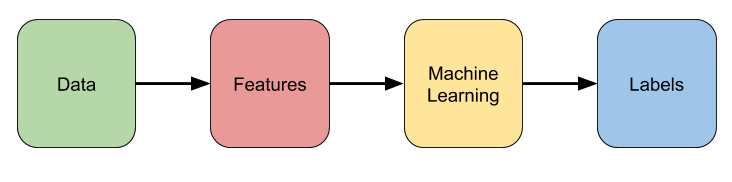
\includegraphics[scale=0.5]{Images/Data-Pipeline.png}
    \caption{Diagram of the Data Pipeline of the project.}
    \label{fig:test}
\end{figure}

When planning and completing this project many decisions were made about the steps taken to convert the raw data to a finished project.
This section may act as an overview of the project, detailing the different sections of work, what they may contain, and the order in which they will be completed.


% Everyone is a question

\subsubsection{Data}

% OLD FROM PROJECT-SPEC


The first component of the project, consisted of extracting the data from it's original JSON format to a csv format.
To achieve this a python script was developed to go through the nested dictionaries unpacking them.

\begin{table}[ht]
    \caption{\label{table:data} The first 5 records of results of the crowdsourced task.
        The table shows the features of the data.
        The lab study data and the crowdsourced data have the same schema, except the lab results have a different ID field.
    }
    \begin{tabular}{llllllll}
        \hline
        event\_type    & target         & time  & x   & y   & step & turkId         \\ \hline
        mousedown      & alloc-slider-1 & 0     & 477 & 405 & 1    & A35YFAFWP33C70 \\
        mouseup        & alloc-slider-1 & 0.111 & 478 & 405 & 1    & A35YFAFWP33C70 \\
        click          & alloc-slider-1 & 0.111 & 478 & 405 & 1    & A35YFAFWP33C70 \\
        mousedown      & alloc-slider-1 & 1.516 & 479 & 405 & 1    & A35YFAFWP33C70 \\
        mousedirchange & alloc-slider-1 & 2.395 & 543 & 403 & 1    & A35YFAFWP33C70 \\
        mousedirchange & alloc-slider-1 & 3.161 & 594 & 402 & 1    & A35YFAFWP33C70 \\
        mouseup        & alloc-slider-1 & 5.048 & 514 & 407 & 1    & A35YFAFWP33C70 \\
        click          & alloc-slider-1 & 5.048 & 514 & 407 & 1    & A35YFAFWP33C70 \\
        mousedown      & alloc-slider-2 & 5.461 & 494 & 441 & 1    & A35YFAFWP33C70 \\
        mouseup        & alloc-slider-2 & 5.513 & 494 & 441 & 1    & A35YFAFWP33C70 \\ \hline
    \end{tabular}
\end{table}

The target field shows which element in Fig \ref{fig:interface} a participant is interacting with and event\_type details the type of interaction.
Time field shows the time taken in seconds since the first recorded mouse event.
We can hypothesise that participants with a shorter time paid less attention than a participant who took much longer, thinking about their actions more.
The x and y fields show the location of the mouse and step shows which stage of the task, from 1 to 5, a participant was in.

% NEW STUFF

% Duplicate or remove to deal with imbalances.
% Probably less effective focusing on this rather than features.

\subsubsection{Data Manipulation}

Here I will summarise what I have done to the data.
As previously mentioned the data was gathered through a lab study and an online crowdsourced study.
The purpose of the online study was to gather a larger amount of data that was possible to do so in person.
% The aim of this was to make any results more statically significant.

Data was recorded in a JSON format with lots of irrelevant and duplicate data relating to the users background and not their mouse movements.
JSON is a form of unstructured data, meaning it is not fully structures but has some organisation to it \cite{ronk2014structured}.
To use the data in this project it first had to be processed into structured data.
This was challenging and time consuming as Python's JSON library was unable to directly convert the data.
This was because the mouse events were stored as a nested JSON dictionary and there were additionally errors with the way the data was logged causing it to be invalid JSON.

After these challenges were addressed the data was converted and saved to a Pandas DataFrame, and then to a csv with over 100,000 lines.
Errors were found in some of the data and so the final number of usable data is less than the amount shown in Table \ref{table:data}.
Example errors include missing mouse events, or time to complete task being recorded incorrectly as 
$1.4 \times 10^{12}$ seconds or $31,688$ years, obviously incorrect.
After removing users will erroneous, or missing data values the quantify of usable data was decreased.
Table \ref{table:UseableData} shows that only 12 of the lab study participants and 361 of the crowdsourced participants data was deemed of an acceptable quality to use going forward.

% TO get percentages we divide the number by 361.
\begin{table}[ht]
    \caption{\label{table:UseableData} The usable amounts of data samples.}
    \small
    \begin{tabular}{llp{2.3cm}ll}
        \hline
        Collection method   & Number of participants & Number of participants with usable data  & Percentage decrease \\  \hline
        Lab study           & 18                        & 12                                    & 33.3\%  \\
        Crowdsourced        & 370                       & 361                                   & 1.9\%  \\  \hline
    \end{tabular}
\end{table}

% TODO: give details on how the data was manipulated form the time in unix time to floats to whole seconds.


% WHOLE section beneath commented out as it wasn't relevant to this section.
% TODO: try and fit in this section elsewhere, but don't know if it will fit.
% This leads to the problem of imbalanced data samples.
% After erroneous data was removed there were only 14 lab data samples and 461 online data samples.
% This means that there were over 30x as many data samples from one class compared to the other.
% As stated in my assumptions, we can say that the lab participants were paying attention, where as the online participants may or may not have been paying attention.

% If the classes were balanced then simple approach may be to treat this problem as binary classification problem.
% Using something like a Support Vector Machine we could classify a given point as lab or online / paying attention or possibly paying attention based on their proximity to other data points.
% To do so we would need to have balanced classes otherwise the algorithm would have a high accuracy from just classifying everything as possibly paying attention as that is the most frequent class.
% However due to the imbalances, alternative methods are required.

% Traditionally there are two main methods of dealing with class imbalances, removing data samples and creating new data samples.
% It was decided that creating new data samples would be best as there is not a whole lot of data to work with, so there would be a strong preference to keep the data we have.
% New points can be created by sampling from a distribution (reference) but here it was decided just to duplicate the samples as there was no discernible distribution of the data.
% Another method is to copy the points, altering them slightly, this was considered but not used in the end.
% Each lab study data sample was copied 40 times to even out the classes.

\subsubsection{Features}
\label{subsection:Features} % Because I reference this section later when creating secondary HMM.

% Tom said something about this being where I should spend the most time of my project.
% Spending time here will be more time effective than other sections.
% This is what people wanna see?
% Evaluating effectiveness of different features.

% What do I so to the raw data.

% What are good features? Big/Good question split into smaller sections.

This part of the pipeline refers to what features I am going to extract from the data.
Features of data can be defined as ``a measurable piece of data that can be used for analysis'' \cite{DataRobot}.
These will consist of both raw and created features, but what do I mean by this?
Raw features will consist of the number of mouse events recorded, while a created feature would have to be extracted from the data.

% TODO: Properly explain how we renamed targets, why
% , and show histograms showing similar distributions of targets.
One such feature recorded in the data is mouse target.
This refers to the HTML element that a users mouse was over at any given time.
As shown in Figure \ref{fig:interface} the most prominent part of the interface that users will interact with is the 5 stock allocation sliders.
% Plot showing alloc-slider-1-5 and other.

It is hypothesised that users who are paying attention may spend more time fine tuning their stock allocation and therefore would have more mouse events with the sliders as the target.
% TODO:
% Talk about how we had to rename the mouse targets with stuff like anything containing the words alloc-slider-1 was renamed.
% Issue with Lab and Turk data having a different naming scheme.
% TODO: Maybe have a table showing the elements name before and after renaming.
An attempt to pick up on different parts of the interface was achieved including which element of the stocks plot a user was interacting with.
However many html elements were ambiguously named and so only the sliders are named from 1 to 5.
% Examples of items renamed are XYZ for the lab data and YZX for the turk data.
% It is obvious that they differ greatly, this is due to differences in how the data is recorded.
% TODO: above

% TODO: TODO: TODO: Normalised Histograms of targets for both classes.
% Say how there are differences in teh averages but that the individuals are more different. 
The html target will be used as a feature in this project.
Additionally a users mouse location over time may provide useful insight into how they completed the task therefore it will also be used.
This feature was even more challenging to engineer as the data needs to be altered to be useful time series of data.

Ideally the data should be given as a multivariate time series which is a sequence of numerical vectors \cite{xing2010brief}.
The data should be in the form
\[    % <-- start math environment
    \langle(t_0, (x_0, y_0)),\; (t_1, (x_1, y_1))\hdots (t_n, (x_n, y_n))\rangle 
\]
where $t$ is the time in seconds, given from the first timestamp $t_0$ in whole seconds to $t=n$.
The tuple $(x,y)$ refers to the horizontal and vertical location of the users mouse cursor.
% TODO: give details on how the data was manipulated form the time in unix time to floats to whole seconds.


\subsubsection{Machine Learning}

% What ML will I do and what algorithm.
% MAybe clustering algorithm but on what data?

Once we have insightful features from the data, we can consider what machine learning algorithm would be most appropriate to use on the data.
This will be highly dependent on what form the final features are in.
For example if the features are numerical values such as time taken to complete task and number of mouse events then an algorithm such as a Support Vector Machine could be a good choice.

If the data is in the form of sequential data such as a sequence of all mouse events then alternative techniques a Hidden Markov Model or neural network would have been appropriate choices \cite{xing2010brief}.
Variations of the traditional neural network such as Recurrent Neural Networks (RNNs) or Long Short Term Memory (LSTM) Networks are known to perform better with sequential data \cite{hochreiter1997long}.
If the features output was an image such as a trace of mouse position over time, then a Convolutional Neural Network could be a suitable choice as they are designed for image data \cite{krizhevsky2012imagenet}.

An issue with any neural network approach would be their tendency to overfit the data.
That is when an overly complicated model tries to model relationships that are a result of noise in messy data.
There is only a limited amount of training data available for this project, and so there is a high risk of this happening.
Despite techniques such as dropout \cite{srivastava2014dropout} existing to address this issue I do not think any form of neural network would be appropriate for this task.
% Could expand lots on why CNNs would be a good choice and also why they weren't used in the end.

% TODO: add somewhere that HMMs can be used as generative models, that might be used in this project somewhere.
% TODO: Another idea: say they can be used to predict the next most probable item in a sequence.
%                       However thats not how they would be used in this circumstance.
%                       Here we would want to see the opposite, what probability a given sequence has of belonging to a model.

It is likely that text classification algorithms will be used when comparing the html targets of mouse events.
Comparing counts of n-grams can be done with algorithms such as probabilistic Naive Bayes classifiers.
Other suitable classification algorithms include proximity-based k-nearest neighbours and ensemble decision tree learners \cite{aggarwal2012survey}.

\subsubsection{Labels}

% Who's paying attention

Lastly an important section of the pipeline, as it reflects the final outputs of the system.
Labels will refer to which users are classified as paying attention and which users are not.

A key aspect of this project will be semi-supervised learning.
That is we have some data points we can confirm were paying attention, and others where they're level of attention was questionable.
Given that it is known that the lab study users were paying attention, the aim is to use this data to relabel some of the crowdsourced data as potentially paying attention.

%Once we have an algorithm that can classify some users as paying attention or not we can rerun the algorithm with these preliminary outputs as new training data.
%If this is done recursively then we can end up with a system that can split all data points into the 2 classes, perhaps with a degree of confidence given as a percentage.


\section{Final Implementation}
% Changed from Implementation to Final Implementation

% Maybe all this should go under the implementation section.

As defined previously a HMM consists of the 5 parameters $(Q,A,O,B,\pi)$ \cite{jurafsky2018speech}.
In the case of this project, the hidden states $Q$ would relate to some aspects of a user's thought processes as that is the behaviour that is being modelled.
The observations $O$ relate to the features as defined in the features section.
Features used are the users mouse location over time and sequence of interface elements.
The parameters $(A,B,\pi)$ are all learned during training, so do not need to be specified \cite{porwal2013machine}.
% TODO: REF https://www.sciencedirect.com/topics/mathematics/hidden-markov-models

Figure \ref{fig:MyHMM} shows the design of the main model used in this dissertation.
It was decided to use only the series of mouse events and ignored the timestamps of the event. % WHY
This is because there was no previous correlation discovered between a user’s total time taken or the number of mouse events. 
Therefore, there is no reason to assume that using a time series would be any more accurate than a non-time series of data. 
The sequence of mouse events should still hold the detail that time data would.

\begin{figure}[ht]
    \centering
    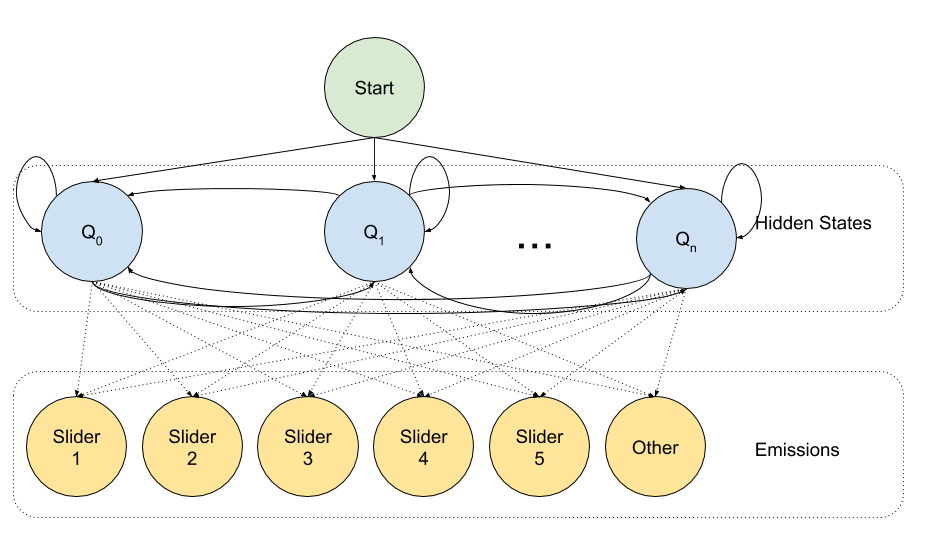
\includegraphics[scale=0.45]{Images/My HMM.png}
    \caption{
        Diagram showing the states of the designed Hidden Markov Model.
        The emissions $O$ are shown to be the mouse targets.
        The number of hidden states $Q$ are not specified as that was decided in Figure \ref{fig:ModleEval}.
        $(A,B,\pi)$ are also not shown as they are calculated and not specified by me.
    }
    \label{fig:MyHMM}
\end{figure}

% TODO: Check that this isnt before I mention bag-of-words models in my diss.
With Bag-Of-Words models the order of items is ignored and only takes into consideration the frequency of each item.
However Hidden Markov Models use a different approach, here the order of the data is the primary attribute the model will use.

% Talk about all different steps you took?
% TODO: Mention the differnt types of HMM, multimodal vs whatever here.
To implement a Hidden Markov Model the python library HMMLearn was used \cite{hmmlearn}.
The MultinomialHMM model was used as the emissions are discrete, representing the different interface targets.
The sequence data used to train the models was the order of mouse targets for each worker.
The temporal aspect of the data was ignored, but earlier research showed that number of mouse events and time were heavily correlated.
Therefore using just the order of mouse events should capture the temporal aspect of the data.

% TODO: Give a much more indepth, mathematical definition of these things.
When implementing a Hidden Markov model on the actual data there are lots of parameters that must be considered. 
Given a sequence of input data the HMM model can calculate the parameters of the model such as the transition matrix, emission probabilities, and initial probability distributions by using the Viterbi algorithm \cite{hmmlearn}.
The most prominent parameter that must be given is the number of hidden states to use.

The issue of selecting a number of hidden states has been addressed with similar data \cite{pohle2017selecting}.
The authors use a HMM to model animal movement behaviour, where they hope the hidden states would roughly relate to the behaviour of the animal.
For example in this context a 2 state HMM may relate to ``foraging/resting'' and ``travelling''.
Humans can be more complex than animals but we can think of potential states of being ``inquisitive'' and ``unengaged''.
They trained models with 2, 3, 4, and 5 hidden states and compared the criterion's of AIC, BIC, ICL.
Similarity to evaluate the Lab and Turk models, several models were trained with number of hidden states ranging from 1 to 11.
Generally, an increase in states should increase the effectiveness, however it will also take longer to train.
All models used for this comparison was trained to 50 iterations for a fair comparison. 

\begin{figure}[ht]
    \centering
    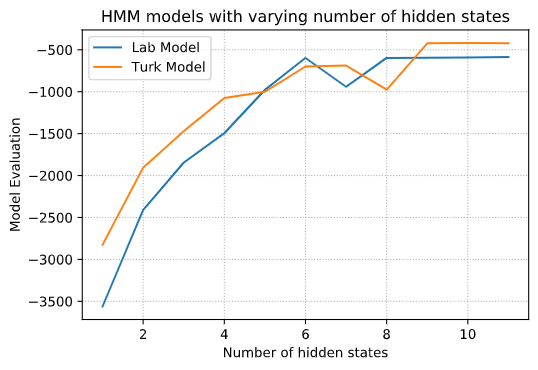
\includegraphics[scale=0.55]{Images/ModelEvaluation.png}
    \caption{Evaluations of different HMM architectures.}
    \label{fig:ModleEval}
\end{figure}

Figure \ref{fig:ModleEval} shows a different criterion of the total log likelihood of the training data of the model.
This is shown on the vertical axis, the horizontal axis shows an increasing number of hidden states of a Hidden Markov Model.
This value is normalised by dividing by the number of data samples, to give a per-sample total likelihood.
The evaluation of each HMM model does fluctuate based on the random state used, which is why there are drops in the evaluation criterion even when more hidden states are used.
We can see that the criterion for both models appeared to stop improving after 9 states.
Therefore a 10 state model was used to ensure that the models could be as accurate as possible while retaining reasonable complexity.

\section{Repeated Experiments}
% Suggested by Tom as an overview of all the work I've done. 

% Commented out all of Repeated Experiments section.
% Not deleted as we might want to take bits from this and copy into other places.
% TODO: Move HMM section out because that section is pretty good.
% NOTE: put back in on 10/09/2020.
% This gave another 1,000 words and will give maybe 2/3x as much as that when all completed.

This section will give an overview of the work I have completed during this project.
Each sub section offers a unique approach to tackling the problem.
The different methods were tried sequentially, and the pipeline had to be amended for each one as the input requirements changed.

The approach of this project was to try many different methods of looking through, classifying, and predicting attentiveness of this data.
These experiments enabled me to get a better understanding of the data, and to explore which methods would be most appropriate.
While these results did not end up directly contributing to the main goal of this paper, they were important steppingstones of the project.

Before any users were reclassified based on their engagement an alternative aim was established.
This was to create a method of identifying whether a user was from the lab study or if they were a crowdsourced turk user based on some input data.
While this is not the ambition of this dissertation, it would reveal information about the two user groups.
If it was trivial to tell these groups apart then it would suggest that there may have been an error in how the data was recorded, or some other unintentional feature a classifier may be identifying.
If any machine learning method was unable to classify a given user then it may suggest that there is little to no difference between the users data.
This could additionally indicate that there is no link between a users mouse data and their engagement, which would be an interesting and surprising discovery. 

% TODO (Get the actual exploration and ml/data science steps by looking at notebooks.)

\subsection{SVM separation method}

% Not sure if this is the best name for it.
This section provided the initial exploration into the problem.
These experiments attempted to separate the data samples for crowdsourced turk users, and lab participants by plotting samples in space.
The aim is that this might reveal information about the features of different users.
If there was a clear distinction between the classes then we could potentially reclassify some points based on their euclidean distance to one another.

A Support Vector Machine (SVM) is a common supervised machine learning technique \cite{noble2006support}.
Here we look at if a simple hyperplane could separate the data when looking at the simple features of the number of mouse events and the total time taken to do the task. 

It was found that a linear, or non-linear classification with a kernel trick was unable to separate the data.
However as shown in Figure \ref{fig:scatterplot}, the data does not appear to be linearly separable.
Regardless this method was still attempted.

\begin{figure}[ht]
    \centering
    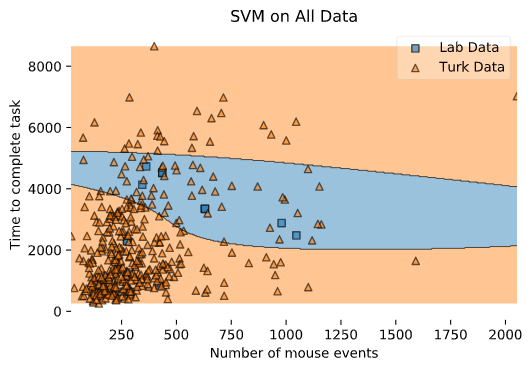
\includegraphics[scale=0.6]{Images/SVM-Decision-Region-Boundary.png}
    \caption{Plot of the SVM, showing the decision region boundary.}
    \label{fig:SVM}
\end{figure}

Figure \ref{fig:SVM} shows the unsuccessful attempts of this method and shows the sheer imbalance of the dataset.
Only 53\% of the lab data was within the relating decision boundary, whereas 86\% of the turk data was in its respective region.
This highlights how this method will be ineffective on the dataset.
While the SVM has created this central band of lab data, this region doesn't accurately model all the data. 

Additionally, this method highlights a reoccurring problem of this project, the unbalanced data classes.
This can make the accuracy of the model high, even if it misclassified most data points.
%[[  8   6]
% [ 53 325]]

%Here simple features of the data was used, the time taken to complete the task, and the number of mouse event taken to complete the task.


% \subsubsection{Clustering}
% Didn't do this but its an example point.
% (Might have tried kNN).

\subsection{Text Classification}

%(Maybe mention bag-of-words models in background research?)
% TODO: I decided on some methods that are used for SPAM detection.

This section of experiments is inspired by text classification algorithms.
Text mining is becoming increasingly popular, due to the large increases in available text data from the web and social media.
Such data is typically unstructured and contains very large amounts of information.
Such data is also sparse and high dimensional \cite{aggarwal2012introduction}.
The high dimensionality of text data stems from the large lexicon of words a document may contain, just the English language has over 170,000 words \cite{BBC2018How}.
Text data is usually sparse because a given document is unlikely to contain anywhere near that many unique words.

The users mouse data used in this project can be represented as an abnormal word document.
% TODO: check that we mention about the mouse targets before, otherwise this will not make any sense.
We can consider a mouse target as a ``word'', and a ``text document'' as a single users sequence of mouse targets.
This data will have a very limited lexicon of only 6 ``words'', the sliders from 1 to 5 and other.
Therefore, this data will have much lower dimensionality than typical text data.
Additionally, every user has interacted with every target, therefore the data is not sparse but dense.

\begin{figure}[ht]
    \centering
    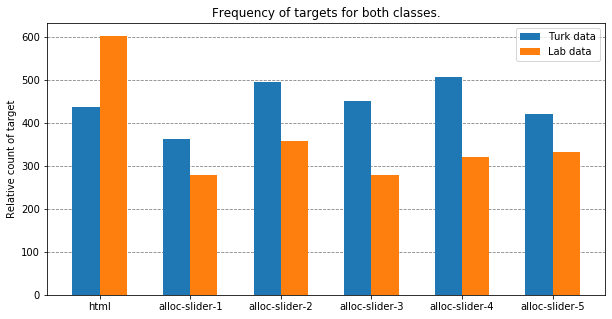
\includegraphics[scale=0.6]{Images/1-grams.png}
    \caption{Histogram of targets.}
    \label{fig:1-grams}
\end{figure}

Figure \ref{fig:1-grams} shows the relative count of each of the targets for the user groups.
The relative count is calculated by dividing the count of the targets by the number of users, this is so the numbers are comparable otherwise the crowdsourced data would be of a much larger quantity.
We can see that lab study users seem to perform more mouse events over the other html elements and not over one of the sliders.
For lab users the most common sliders are 2, 5, then 4.
For turk users they are 4, 2, then 3.
The causes of these differences are unknown.
Importantly they show that there are differences in the data from the classes, something that a classifier should be able to exploit.

% FROM THE CODE
% TODO: Add to this section if I want more depth in this section.
% Normally with Bag-Of-Words models we end up with a spare matrix of mainly 0s. 
% https://machinelearningmastery.com/gentle-introduction-bag-words-model/
% However becuase our vocabulary is so limited (only 6 'words') the martix is full 
% and so we dont have to wory about effeciency.
% TF-IDF will not work due to small vocabulary.
% Word hashing is used to help complexity but this is simple enough that we dont need it.
% ALSO TODO: Add talk about the CountVectoriser and how it creates the feature vectors.

% TODO: Add plot of number of targets normalised for both groups
% df_lab['target'].value_counts().plot(kind = 'bar') divided by num of users.

One popular text classification method is with a Bag-Of-Words model, called such because the grammar and order of the words is ignored and only the counts of each word is used as a feature \cite{jurafsky2015text}.
Grammar is meaningless in the context of mouse data, however the sequence of the words may hold crucial information regarding what class a user is in.
Disregarding the sequence may be a big limitation of this method as we can imagine a user switching between sliders frequently may be very engaged in the task.
Therefore disregarding the order of targets could be detrimental to the model.
The Bag-Of-Words representation of the data can be used as input to a Naïve Bayes classifier \cite{jurafsky2015text}.
A Naïve Bayes classifier predicts a class based on the probability of seeing the counts of words in a document.  
It can potentially be used here to classify users as lab study or crowdsourced based on their counts of targets.
For example it may be found that crowdsourced turk users may have a higher lower counts for the later targets, potentially showing how they got tired of the task and stopped putting effort into it.

\[    % <-- start math environment
\begin{pmatrix}
    322 & 430 & 464 & 308 & 230 & 1317 \\
    332 & 120 & 112 & 123 & 59 & 164 \\
    41 & 367 & 173 & 565 & 278 & 449 \\
    \vdots & \vdots & \vdots & \vdots & \vdots & \vdots \\
\end{pmatrix}
\]    % <-- end of math environment

\bigskip % to skip a line
This matrix shows the first 3 rows of the bag of words representations of each users data.
The matrix has 6 columns representing each of the mouse targets or ``words''.


% TODO: Model results here.
% TODO: Do k-fold cross validation to keep class size the same.
This attempt of classification was a failure.
The accuracy was 29.6\% and F1 score of 22.8\%.


% TODO: Use these references about dealing with imbalanced data in diss.
% https://machinelearningmastery.com/failure-of-accuracy-for-imbalanced-class-distributions/
% This website has some nice references about imbalanced class distributions.
% ( TODO: use in diss)
% data sampling – customized algorithms– cost sensitive algorithms– one class algorithms – threshold moving – probability calibration

% $https://machinelearningmastery.com/tour-of-evaluation-metrics-for-imbalanced-classification/$
% Better ways of dealing with imbalanced data

\subsubsection{N-Grams}

The previous Bag-Of-Words method would be considered an unigram model of natural language processing.
An n-grams is a series of n words, with unigrams being one word, and bigrams being two word pairs \cite{keselj2009speech}.

Different n-grams can be combined together to better understand the complexities of a text document.
A mixture of unigrams, bigrams, and trigrams are used extract different levels of text complexity and perform well with document classification \cite{aggarwal2012survey}.
The same technique can be applied to this mouse dataset.
Bigrams will be of interest as they show the transitions from one target to another, thus adding some sequential data to be used by the model.
However higher n n-grams could reveal information about a users approach to the tasks.
A user who has many n-grams of different sliders would mean they often changed between sliders, potentially looking for the optimum slider values.

\begin{figure}[h!]
    \centering
    \begin{subfigure}[c]{0.4\linewidth}
        \centering
        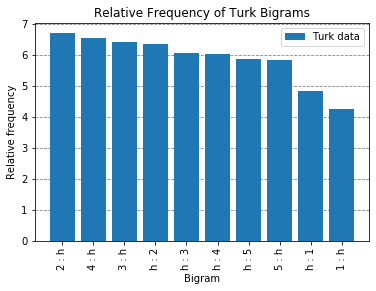
\includegraphics[scale=0.55]{Images/turk-bigrams.png}
        \caption{Turk Bigrams}
    \end{subfigure}    
    \hfill
    \begin{subfigure}[c]{0.4\linewidth}
        \centering
        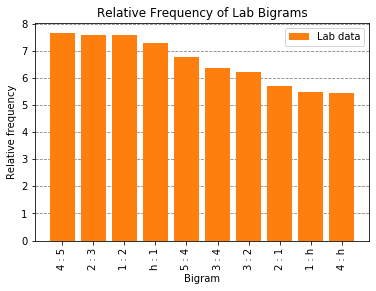
\includegraphics[scale=0.55]{Images/lab-bigrams.png}
        \caption{Lab Bigrams}
    \end{subfigure}  
    \caption{Plots showing the relative frequency of bigrams for both groups.}
    \label{fig:bigrams}
\end{figure}

Figure \ref{fig:bigrams} shows the bigram differences of the crowdsourced turk data and the lab study data.
By far the most frequent form of bigram was the same target followed by the same target.
This indicates that if a user is using a slider their next target will most likely be the same slider, which intuitively makes sense.
To address this issue bigrams leading to themselves were excluded from the visualisation.
There are 36 unique bigrams, however only the top 10 most frequent bigrams are shown.
We can see that the turk data is more likely to have a html element somewhere in the bigram, whereas lab users are more likely to have just have sliders.
This is surprising as in Figure \ref{fig:1-grams} it was shown that a html target was more common in the lab study data.
The plots show how bigrams can be used to separate the data, it is hoped that this may help classification especially when combined with trigrams.


% TODO: Do with n-grams from 1-3 and see how many columns there are.
With a combination of unigrams, bigrams, and trigrams the matrix now grown massively to have a total number of 222 columns.

% TODO: cross validatoin.
However due to the problems there is still an accuracy of 94.9\% and an F1 score of 48.6.

\subsection{Imbalanced classes}

% Someone's dissertation on the topic of generating synthetic data with HMMs.
% This can be a good way to create synthetic data \cite{ferrando2018generating}.

% Hidden Markov Models are generative models.
% They model the most likely output sequence  \cite{ibe2013markov}.


As detailed previously HMMs can be used for classification, but they are also known as generative models \cite{ferrando2018generating}.
This means they can be used to create new data.
This is promising as the previous methods of Bag-Of-Words and N-grams failed due to the imbalances of classes.

There are many methods to address the issue of class imbalances.
Class imbalances involve a minority class (in this case lab study data) and a majority class (in this case crowdsourced turk data).
Two of the most popular solutions are to over-sample the minority class or to under-sample the majority class \cite{chawla2002smote}.
In there basic forms under-sampling effectively ignores data from the majority class, and over-sampling effectively duplicates existing data.

It was decided that under-sampling would not be appropriate as there is only a small amount of data, therefore as much data must be kept as possible.
Over-sampling was a better solution however, to balance the classes the number of samples must still be increased by around 20 times as much. 
Trained intelligent undersampling methods can perform better but are more difficult to implement \cite{chawla2002smote}.
Therefore it was decided to use the existing Hidden Markov Model to generate new data.
A trained HMMs can be used to generate new data points, to reduce the imbalances, and make the previous classification methods more effective.

A HMM can be used generate a probable sequence of $n$ observed states, however to generate new samples we must decide what length n must be.
Given $n$ a walkthrough of the model is performed, the transitions between states then occur based on the probabilities within the transitional matrix.
The idea of this section is to generate new lab study data so that there is the same quantity of lab study data and crowdsourced turk data.
This generated data can be used to train the models used previously with the hope that this new data will address the issue of unbalanced data.
The turk data and the generated data will be split into training and testing data as standard.
However, the original lab data will not be used to train the model, this will be withheld to see if the models trained from the generated data will be able classify the actual lab data.

\begin{figure}[ht]
    \centering
    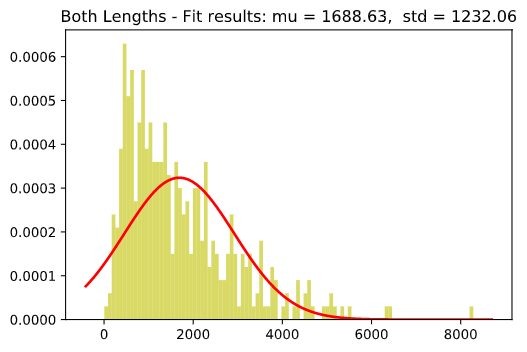
\includegraphics[scale=0.5]{Images/Lengths-Histogram.png}
    \caption{Histogram of length of mouse events sequences for both groups.}
    \label{fig:normaldis}
\end{figure}

Figure \ref{fig:normaldis} shows the frequency of different mouse events lengths.
In red we can see a positively skewed normal distribution which matches the distribution fairly well.
When determining n for the new sequence data, we will sample from a gaussian distribution with a mean of 1688 and a standard deviation of 1232.
This should generate a realistic distribution of lengths, and when combined with the trained HMM model, a realistic sequence of data.

%TODO: Check why this number is different from the other number of turks.
From this distribution 378 values were sampled.
Each of the 378 values were then passed into the generative lab study HMM.
This led to the creation of an equal number of crowdsourced data and synthetic lab data generated from the model.

\subsubsection{Revisiting methods}

% This section will discuss the generative properties of a HMM.
% Explain how the lengths were modelled as a gaussian and points sampled form there.
% This enables us to, in a way, address the earlier concerns of imbalanced data sizes.
% TODO: Reference paper that says one way to address imbalanced data is to generate new data.

% Then in conclusion say that while there are definitely issues with the way I created data from such a small number of samples.
% However it is nice to see that the methods developed earlier in the project are successful, and are appropriate.
% They were just held back by the poor quality of data which was addressed as one of the major shortcomings of this project.



With the generated lab study data we can now revisited some of the methods that failed due to imbalanced classes.
The SVM classifier was unable to be revisited as the features used before were the time taken to complete the task and length of mouse events sequence.
The generated data has a length, however there is no corresponding time feature.
Despite the data not being suitable for a similar SVM the data was perfect for the previous Bag-Of-Words methods.

Using the Naive Bayes classifier with a Bag-Of-Words methods, there was improvement.
The model was trained and tested with 5-fold cross validation which led to an accuracy and f1 score of 60\% and 58\% respectively.
% Compare this to k-fold CV of non generated data.
When the bigram model was considered the accuracy increased by 1\% to 61\% and the F1 score remained the same. %45% seems low, rerun.
Additionally using the original lab study data as testing led to the same results from both models with the same confusion matrix.
% TODO: Put confusion matrixes everywhere.
\[    % <-- start math environment
\begin{pmatrix}
    0 & 0 \\
    2 & 12 \\
\end{pmatrix}
\]    % <-- end of math environment

The confusion matrix from the models shows that of the 14 original lab study participants, only 2 would be misclassified as a crowdsourced participant.
This shows that there is enough difference in the data for a classification algorithm to distinguish the points. 

\section{Results}
% talk about results
% Should I talk about all the results, or just the end results that I feel are conclusive.

%Now the real aim of the project can begin, attempting to classify users as paying attention or not.
Hidden Markov Models were trained on both lab study users mouse data and online crowdsourced mechanical turk mouse data.
Then each users mouse data was evaluated by each HMM, and the log Likelihood of that sequence belonging to that model was recorded. 
This will tell use the likelihood that that sequence of mouse events belongs to either of the classes.
If there are any points that appear to be outliers, then we can say that they were doing something differently to the majority of their peers.
Outliers with a higher likelihood of belonging to the HMM trained on data from the other group then we can say that that outlier sample appears to belong to the wrong group.
Or at least that outlier is doing something different to their peers, which may be a higher level of attention given to the task. 
These points were labelled Reclassified Lab data and Reclassified Turk Data.

\subsection{Graphs of results}
% Plot histogram of likelihoods for both classes on both HMM models.
% Examine outliers.

One way of attempting to classify users is to identify any users with a higher lab likelihood as being more similar to a lab user than a turk user.
Figure \ref{fig:unreclassified} shows this result graphically.
Any data point above the line $y=x$ has a higher likelihood of belonging to the lab model than the turk model.
Therefore any turk data that is above this line can be reclassified as seeming to belong more with the lab data than the fellow turk datapoints. 
An interesting and surprising result is shown from the lab data.
Not all of the lab data is shown to be belonging more strongly to the lab model than the turk model.
6 out of 14 (43\%) of the lab data samples has been reclassified by the algorithm as being more similar to the turk data.

\begin{figure}[ht!]
    \centering
    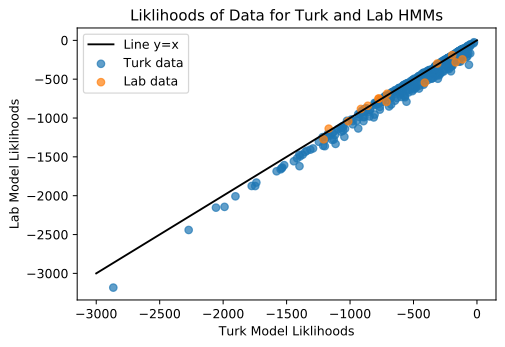
\includegraphics[scale=0.5]{Images/labturklikli.png}
    \caption{Scatterplot of users likelihood of belonging to either group. }
    \label{fig:unreclassified}
\end{figure}


\begin{figure}[ht!]
    \centering
    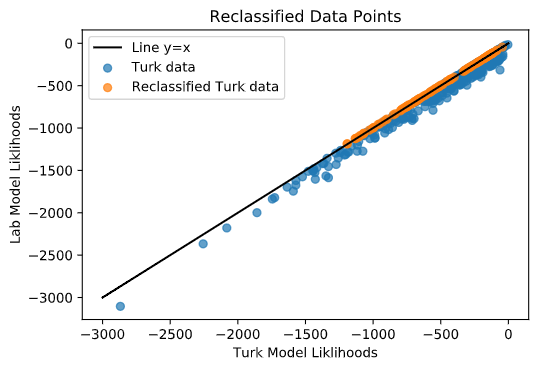
\includegraphics[scale=0.5]{Images/Reclassified-Data.png}
    \caption{Scatterplot showing the turk users that have been reclassified as behaving more like lab users. }
    \label{fig:Reclassified}
\end{figure}

Figure \ref{fig:Reclassified} shows which of the turk users are more similar to the lab users, than other users from the same group. 
The plot shows the same datapoints and axis as in Figure \ref{fig:unreclassified}, but the points above the line are recoloured green to show their difference from the actual lab data and normal turk data. 
45 of the 361 (12.5\%) turk users are above this threshold. 
Which seems like a reasonable percentage of the population to be paying attention. 

% TODO see if I can find any references that say how many turkers/anyone pay attention at a given time.
The exact distribution of these points change based on the initial random state when training the model.

Figure \ref{fig:scatterplot} showed a naive simple attempt to separate the classes of turk users and lab users.
It was concluded that a spacial based technique such as a SVM would be unsuitable as the data didn't seem to form any patterns or clusters.
Figure \ref{fig:Reclassified-Scatterplot} shows how the reclassified datapoints are not linearly separable.
This proves that my initial hypothesis was correct, and that data could not be reclassified purely by looking at simple feature of time taken and just number of mouse events.

% TODO fix labels, this shows reclassified turk/lab data and the unclassified samples.
\begin{figure}[ht!]
    \centering
    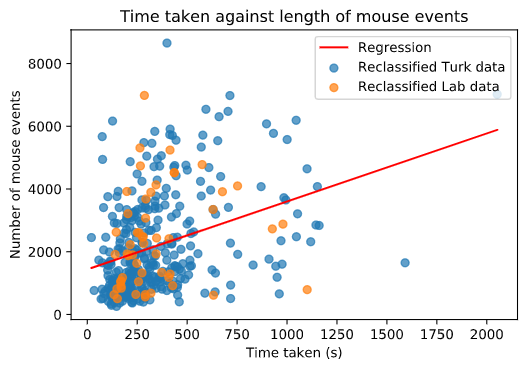
\includegraphics[scale=0.5]{Images/TimeTaken-Mouse-Events-Reclassified.png}
    \caption{Plot showing features of the reclassified points. }
    \label{fig:Reclassified-Scatterplot}
\end{figure}

\subsection{Likelihood length correlation}

Examination of the extreme points with the highest and lowest likelihoods revealed a potential correlation likelihoods and length of mouse events sequences.
I decided to plot this data to understand if there was a link between these features.

\begin{figure}[h!]
    \centering
    \begin{subfigure}[c]{0.4\linewidth}
        \centering
        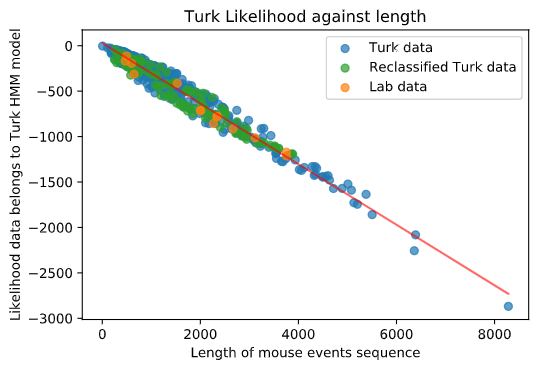
\includegraphics[scale=0.4]{Images/Turk-Liklihood-Length.png}
        \caption{Turk HMM Model}
    \end{subfigure}    
    \hfill
    \begin{subfigure}[c]{0.4\linewidth}
        \centering
        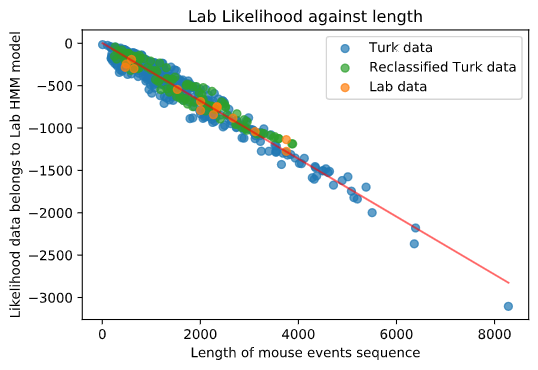
\includegraphics[scale=0.4]{Images/Lab-Liklihood-Length.png}
        \caption{Lab HMM Model}
    \end{subfigure}  
    \caption{Plots showing correlation between likelihood of different models and the length of mouse events.}
    \label{fig:liklihoodlengths}
\end{figure}

Figure \ref{fig:liklihoodlengths} show that the log likelihood from both models and length of a users mouse sequence are highly inversely correlated. 
The Lab model likelihood and length have a correlation of -0.982, and similarly the Turk model has a correlation of -0.976.
A value less than $-0.7$ would indicate a strong negative correlation, therefore Figure \ref{fig:liklihoodlengths} shows an extremely strong negative correlation \cite{mindrila2017scatterplots}.
Such a strong correlation could indicate the models are doing nothing, other than looking at the length of a sequence.
However looking at the reclassified Turk data we can see that there doesn't appear to be any correlation between length, and whether the data has been reclassified.
Therefore such a strong correlation between the length and likelihood is of no concern. 

\begin{figure}[ht!]
    \centering
    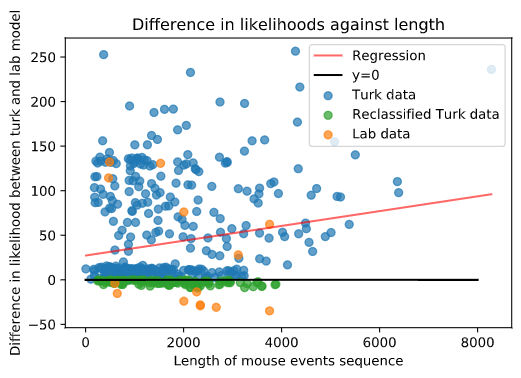
\includegraphics[scale=0.5]{Images/Difference-Liklihood-Length.png}
    \caption{Plot showing difference in likelihood between the models against length of mouse events sequence. }
    \label{fig:diffliklihoodlengths}
\end{figure}

Figure \ref{fig:diffliklihoodlengths} removes the concern that length of mouse events sequence is the only feature being used in the models.
The difference in likelihoods and length of mouse events sequence has a correlation of $0.176$, meaning the relationship between the features is non-existent.

% Think of better model than secondary model.
\subsection{Secondary Model}    % Changed from Further Results section to Secondary HMM sub section
% In this section I will talk about how the additional secondary HMM was created to confirm the results.
% Maybe double check with other HMM using mouse location data.
% Stretch goal as I don't think this adds much other than saying I can make another HMM but with completely different results.
% This section says the above is still the final results, but these 6 users are of particular interest. 

% Information copied from HMM cursor location

In order to confirm any findings, it was decided to attempt another experiment using similarly designed HMMs.
The key difference is that these models will be trained with different data than the previous models.
If models are created with different data, but they identify the same users as potentially belonging to the wrong group then it would be a confirmation that those users are indeed outliers.
If the models predict a completely different group of users then it would indicate there is no consistency within the data and that the models may not be reflecting the actual processes.  

% TODO:fFind reference that HMMS are good at spatial data.

The initial ideas was that confirmation models would be trained on multivariate time series as described in Subsection \ref{subsection:Features} Features.
However using a time series of data caused too much variance in the results, meaning that it could not be modelled by a Hidden Markov Model without access to more data.
Therefore the sequence of mouse locations was used instead which can still provide interesting results as shown with the other model.
Because of the different data this model will be a Hidden Markov Model with gaussian emissions as the multivariate inputs are continuous.

The reason that this data is only a secondary aspect of the dissertation is due to concerns with the quality of data.
Particularly that the mouse location data does not seem to be calibrated correctly.
Looking at the mouse cursor position for each position it would be expected that many of the cursor locations each user would be the same.
For example, you would expect to see 5 distinct clusters of intensive mouse activity relating to the 5 allocation sliders.
To end the task workers must press a ``Buy'' button to purchase their selected stocks.
Therefore, the last recorded mouse event of all users should have the same position, that of the button.
% TODO: Show plot of last event of every user, will NOT show the same position.
Unfortunately, this was not the case.

\begin{figure}[ht!]
    \centering
    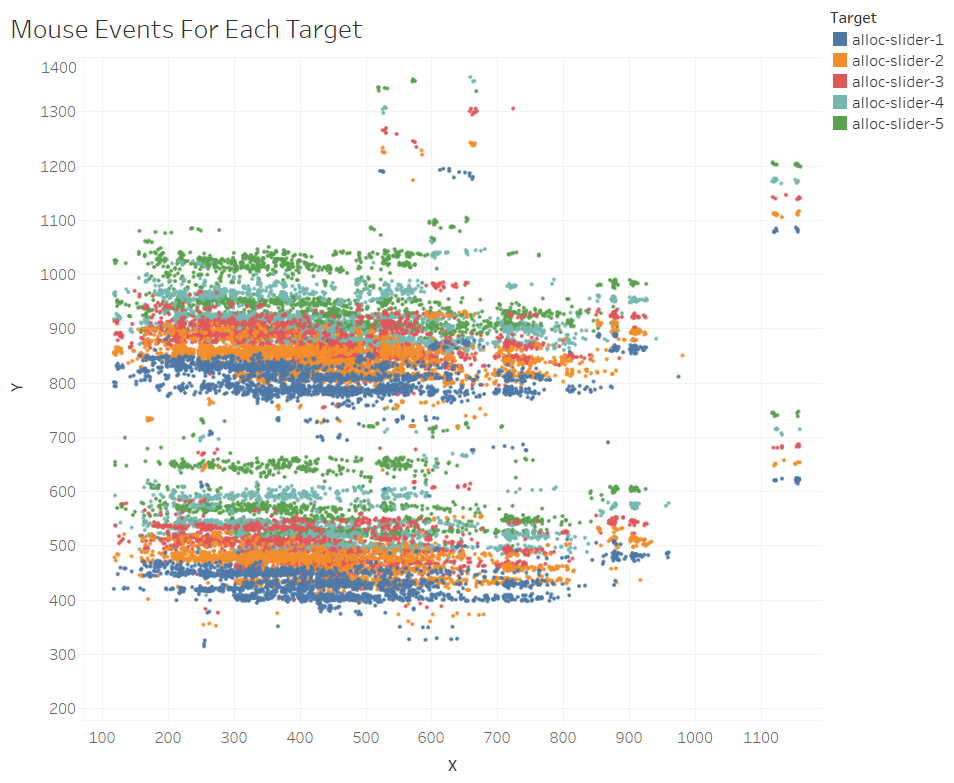
\includegraphics[scale=0.65]{Images/Mouse-Events-For-Each-Target.png}
    \caption{Scatterplot of mouse down event coordinates of all users mouse path data.}
    \label{fig:MouseEventsTargets}
\end{figure}

Figure \ref{fig:MouseEventsTargets} shows the issues with the mouse location data.
Rather than the mouse events for the sliders having roughly the same there appears to be multiple groups with varying coordinates.
The majority but not all of mouse down events happen within two groups with the same y coordinates. 
Additionally there is a massive range in mouse data.
Most data falls below an X value of 800, and most are beneath a Y value of 1000 however there are still outliers to this.
Figure \ref{fig:MouseEventsTargets} shows only the mouse down events on the slider targets, when considering the other mouse events and other targets the data was even more messy. 
The cause of this is unknown but is expected to be a result of the data recording process.
% TODO: If I have time Id love to normalise each users events

This messiness of this mouse data was not addressed.
This is the reason that this method will only be used as a supporting secondary model.
It is impossible to draw concrete conclusions from such messy data.
This data may cause some of the users data to be unlikely to belong to any model as they’re such a large outlier.

\subsubsection{Results}

\begin{figure}[ht!]
    \centering
    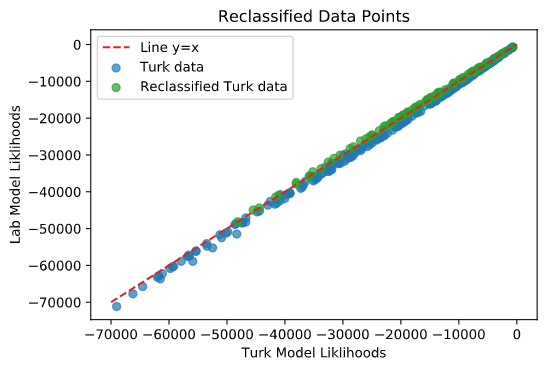
\includegraphics[scale=0.5]{Images/Spatial-Reclassified-Data.png}
    \caption{Graph of reclassified datapoints from spatial data HMMs.}
    \label{fig:SpatialRecData}
\end{figure}


Figure \ref{fig:SpatialRecData} shows how the new HMMs reclassified 80 of the crowdsourced turk users as belonging more to the lab study.
It is worth noting that the likelihoods of each user belonging to the model is much lower when the spatial data is used, 
compared to when the mouse target data was used.
This is because there is much more variance in the continuous spatial data rather than the categorical target data.
The original previous HMM classified 45 of the crowdsourced users.
Taking an intersection of the sets of users will highlight the consistency, or inconsistency of the results.
If there is a large intersection of users then the results are consistent with the previous model, however if there is little to no intersection then it would indicate that there is no consistency between models. 

% Remove equation
%${Previous Reclassified Users} \cap {New Reclassified Users}$

There is an intersection of 12 users between the two sets of users.
This indicates either that there is some consistency in the results.
27\% of the originally reclassified users were identified by the secondary model. 
% TODO: Maybe do some research into how to compare 2 subsets of the same data.
% 80/461 = 0.174
This is promising as it shows that a number of the reclassified users are shared between both methods.
% Say what I'm trying to say much better.
The inconsistency in the mouse location data identified could be causing the differences in reclassified users between the methods.
Therefore I would predict that the results from the spatial models to be less accurate and representative of the real world processes that the models trained with mouse target data. 

If we take the union of both sets of reclassified users we get a set of 184 reclassified users.
This allows us to have a few different sets of users that we may reclassify as belonging to the wrong group, with different confidence levels.
I am most confident in saying that the 16 users reclassified by both versions of the models seem more similar to the lab study users than the other crowdsourced users.
I am next most confident in the 42 users reclassified by the HMM trained with mouse target data.
This is because data used in those models was more properly cleaned and had less variation in data.
The users I am the least most confident in reclassifying is the union of users from both sets of models.
This consists of 184 crowdsourced users which is over half of the total population.

% TO get percentages we divide the number by 361.
\begin{table}[ht]
    \caption{\label{table:usersattention} The different sets of crowdsourced user paying attention with confidence.}
    \small
    \begin{tabular}{llll}
        \hline
        Number of Users & Percent of Population & Identified By Models             & Confidence Level \\  \hline
        16              & 4.4\%                 & Both Models                      & High  \\
        42              & 11.6\%                & Target Data model only           & Medium  \\  
        184             & 50.9\%                & Cursor Location Data model only  & Low  \\  \hline
    \end{tabular}
\end{table}

% Removed as it was confusing and the confidence number pairs were wrong and I didnt like  it
% Alternatively inverting this gives us users which we can assume are not engaged in the tasks, to different degrees.
% I am most confident in saying that 177 of the crowdsourced users not reclassified by either models belong with their class, and were potentially not paying attention.
% I have next most confidence in the 319 users that were identified with the mouse target data models.
% Lastly we have the 345 users not identified by the intersection of both models.
% I am least confident in saying that these users were not engaged in the task.

\section{Future work}

All the problems addressed in the conclusion have potential to be addressed in future work.
% TODO: Write order of future work based on the order of the conclusion.
As stated the main flaw of this project is that the label is not labelled for the task I am trying to perform.
% Taken from abstract
Therefore to fully evaluate any of these results would require further research with a properly labelled dataset.

% While it was hypothesised that differences in mouse data from users using both 

It was hypothesised that a users mouse data would not be significantly different depending on which version of the study interface they were using.
This hypothesis was based on the findings of the previous study, where the different interfaces had little to no impact on a users success at the investment scenario \cite{gruber2017thesis}.
Perhaps an investigation into users mouse data might show more of a difference between the behaviours of users using both interfaces.

% TODO: Expand on how and why 'RONA fucked up these plans.
I would have liked to perform an additional lab study session where we could have generated more data for that class of participant.
This would have helped alleviate the issue that the imbalance of classes caused.
Unfortunately, this was impossible due to time restraints and the interference of the global COVID-19 pandemic.

Another area of future work would be to see if any of the methods developed here could be applied to other similar datasets.
A kaggle crowdflower dataset seems like an idea candidate \cite{kaggleWorkerActivity}.
While it is still not labelled with attention and non-attention, it does contain mouse data of crowdsourced users.
Additionally the dataset contains the users results from 3 different tasks, a users success at a task may prove to be a reasonable proxy for engagement. 

% https://www.scribbr.co.uk/thesis-dissertation/conclusion/
% 5-7% of word count 
\section{Conclusion}

This dissertation aimed to detect user engagement from mouse tracking data.
From the analysis and exploration conducted it cannot be fully concluded that the methods presented here can fulfil this aim.
The initial results are promising, but without a properly labelled dataset there is no way of confirming these results.

To summarise this project users mouse data from two groups of users performing a simple task was analysed and modelled.
The different groups conducted the experiment in different ways.
18 of the participants conducted the experiment in a lab, where they were closely monitored to ensure they were paying attention.
370 of the participants were crowdsourced online using Amazon’s Mechanical Turk.
These were not monitored so it is uncertain if they were paying attention.
However due to erroneous data not all of the data from these participants could be used.
% TODO: Double check these numbers I just made them up

The main goal of this dissertation was to identify which of the crowdsourced users may have been paying attention.
A variety of techniques was attempted, and the use of Hidden Markov Models was evaluated to perform best at this task.
Models were trained for each group of users on different sources of data. 
One a sequence of html element targets and the other a multivariate series of a users mouse cursor location.

Each user's data was evaluated on the lab model and the crowdsourced turk model.
Some of the crowdsourced users was evaluated to belong more closely to some of the lab study users rather than the other crowdsourced users.
This means that these users were doing something different from their peers, they are suspected to be paying attention more than their peers. 
From the results of the model I can predict that anywhere from 184 to 16 of the crowdsourced users were paying attention, with varying degrees of confidence.

% Older conclusion
However I would not be too confident in my findings.
The data was incorrectly labelled for the task I wanted to perform.

The data was heavily imbalanced, there is a comparatively very small volume of lab study data compared to the crowdsourced data.
All of the conclusions I have made from the lab data are relying on only a small number of datapoints which is not statistically significant.
There were not meaningful amounts of data from the other class of crowdsourced data either.
Typically, data science and machine learning uses big data, where as this project used only 388 records in total which came to only 330 MB of data in its original JSON format.
Any bias in any of these original samples will be magnified as this was used to classify more points, which would spread this bias.
% This would become a self-fulfilling prophecy as more similar points would be labelled and spread the belief.

Another potential flaw of the project is the first assumption, that the lab study participants were always engaged.
While they were monitored and we can be sure they were not distracted by items such as phones or televisions, many of them may have 'zoned out' and not have been given it their full effort and attention.

Any concern that the models have learned of a simple feature such as sequence event has been disproven, showing the reclassification algorithm does not model a simple relationship.

To conclude further work is required to strengthen the findings of this dissertation, although the initial results do appear to be promising.

%\subsection{Revisiting methods}
% Then in conclusion say that while there are definitely issues with the way I created data from such a small number of samples.
% However it is nice to see that the methods developed earlier in the project are successful, and are appropriate.
% They were just held back by the poor quality of data which was addressed as one of the major shortcomings of this project.


\singlespacing
\printbibliography

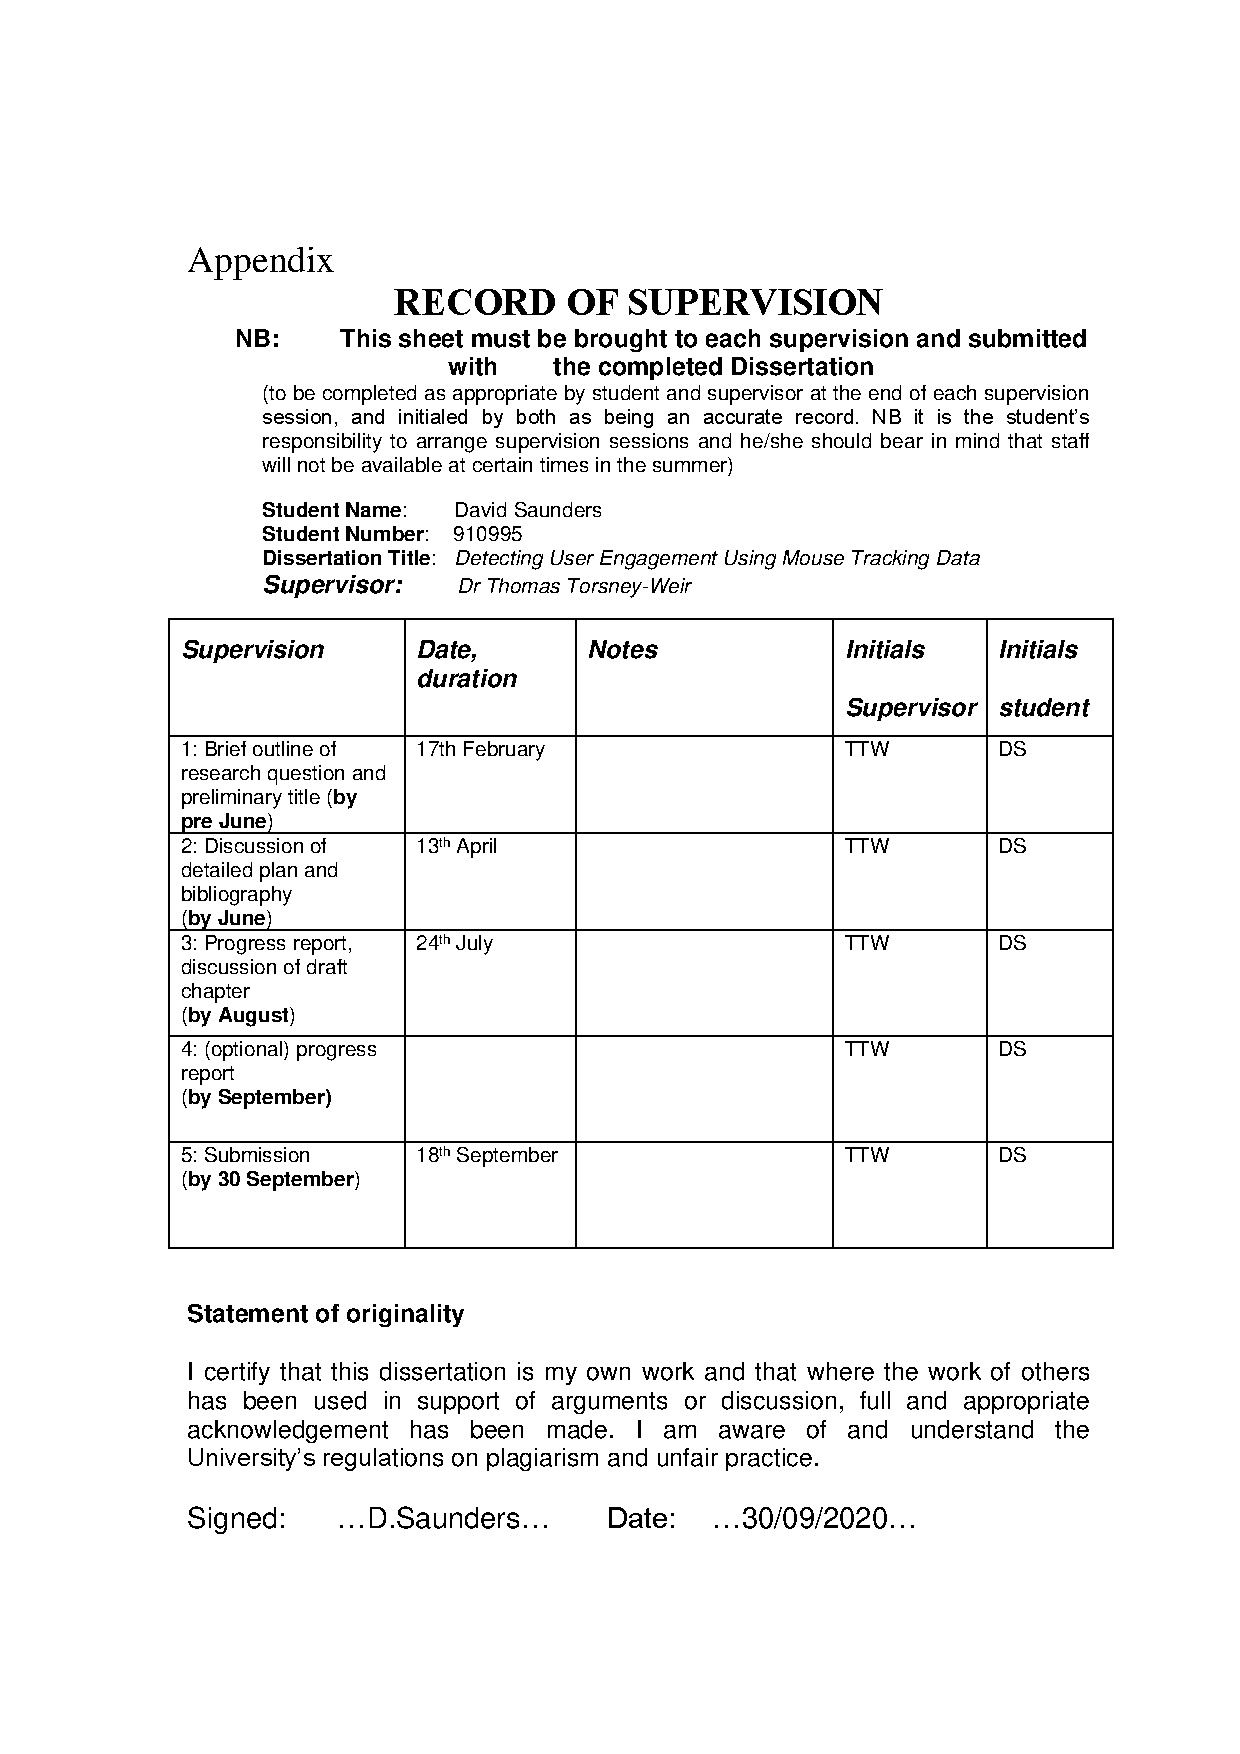
\includepdf[pages={1}]{Declaration/RecordOfSupervision.pdf}

\end{document}